\documentclass[12pt]{article}
\usepackage[utf8]{inputenc}
\usepackage[T1]{fontenc}
\usepackage[italian]{babel}
\usepackage{graphicx}
\usepackage{float}
\usepackage{listings}
\usepackage{xcolor}
\usepackage[a4paper, total={17.5cm,24.7cm}]{geometry}
\usepackage{parskip} % Skip indentation after new paragraphs

% Definizione dello stile per il codice JSON
\lstdefinestyle{json}{
    basicstyle=\ttfamily\small,
    commentstyle=\color{green},
    keywordstyle=\color{blue},
    stringstyle=\color{red},
    breaklines=true,
    showstringspaces=false,
    % frame=lines,
    captionpos=b,
    xleftmargin=3em % Imposta il margine 
}

\title{Peer-Review 2: Network}
\author{Samuele Allegranza, Matteo Arrigo, Lorenzo Battini, Federico Bulloni\\Gruppo AM13}



\begin{document}

\maketitle

\section{Introduzione} %Dettagli comuni radice tra Socket e RMI
Per gestire l'aggiornamento delle \texttt{View} di ogni giocatore in seguito a una modifica dello stato della partita (\texttt{GameModel}) abbiamo applicato il design pattern \texttt{Observer} (che noi abbiamo chiamato Listener per semplicità). Nella nostra implementazione un \texttt{GameListener}, che corrisponde in maniera univoca a un giocatore/client, viene aggiunto alla lista di giocatori (\texttt{ListenerHandler}) interessati a ricevere aggiornamenti sullo stato della partita (\texttt{GameModel}). In questo modo ogni volta che lo stato della partita viene modificato, la classe GameModel si occupa di chiamare il corrispondente metodo di \texttt{notify()} di ListenerHandler che a sua volta richiama il corretto metodo di \texttt{update()} di GameListener. Essendo quest'ultima un'interfaccia, la classe che la implementa avrà totale libertà su come descrivere i metodi \texttt{update()}, che dovranno aggiornare lo stato della partita che risiede sul client e la sua View.
\\
Abbiamo scelto di implementare le funzionalità avanzate "Resilienza alle disconnessioni" e "Partite multiple". 
\section{Socket}
Il \texttt{ServerMain} resta in ascolto della connessione di nuovi client, effettuando il binding e poi istanziando \texttt{ClientRequestsHandler} che si occuperà di tutte le successive comunicazioni in ingresso da tale client.
\\
Tutti i messaggi sono trasmessi in formato json.
\\
I messaggi sono trasmessi dal server al client tramite \texttt{ListenerHandler} in broadcast. In particolare, ad ogni azione nella view del client corrispondono una o più notify, che chiamano i metodi update su ciascun \texttt{GameListenerServerSocket}.
\\
Fa eccezione solamente \texttt{getRooms()}, dato che tale richiesta è la prima ad essere chiamata, quando ancora non è stato scelto il nickname da parte del giocatore e non è ancora stato creato il \texttt{GameListenerServerSocket} ad esso associato. In questo caso la risposta viene quindi inviata da \texttt{ClientRequestsHandler} al client che ha mandato la richiesta.


\newpage
\subsection{Messaggi}
I pacchetti scambiati tra server e client si differenziano in messaggi \textbf{command} e messaggi \textbf{result}.

\begin{itemize}
    \item I messaggi \textbf{command} sono inviati dal client al server e corrispondono ad un comando che deve essere eseguito sul server. Ogni messaggio command ha associato il nome del giocatore. Un messaggio command provoca l'invio di un messaggio result da parte del server.
    \item I messaggi \textbf{result} sono inviati dal server a tutti i client partecipanti di una specifica partita e generalmente corrispondono alla risposta di un messaggio command inviato da un client specifico.
\end{itemize}

Pertanto, se un client invia un messaggio command, la risposta result non verrà inviata solamente al chiamante, ma anche a tutti gli altri giocatori.
Se l'operazione richiesta da un client mediante messaggio command non è valida, viene inviato un messaggio result contenente un errore al solo client richiedente.

Riportiamo di seguito la struttura comune per i messaggi command:
\begin{lstlisting}[style=json]
{
    "command" : COMMAND_NAME,
    "nickname : NICKNAME,
    "body" : {
        COMMAND_BODY
    }
}
\end{lstlisting}

Riportiamo di seguito la lista dei tipi di messaggi command che possono essere inviati. Ognuno avrà un body (\texttt{COMMAND\_BODY}) diverso che contiene le informazioni strettamente necessarie per la richiesta.

Messaggi command di gestione della Room di gioco:
\texttt{
\begin{itemize}
    \item getRooms
    \item createRoom
    \item joinRoom
    \item leaveRoom
\end{itemize}
}

Messaggi command di gestione del flusso di gioco:
\texttt{
\begin{itemize}
    \item playStarter
    \item choosePersonalObjective
    \item playCard
    \item pickCard
\end{itemize}
}

Messaggi command di gestione della connessione di rete:
\texttt{
\begin{itemize}
    \item ping
    \item reconnectGame
\end{itemize}
}

Riportiamo di seguito la struttura comune per i messaggi result:
\begin{lstlisting}[style=json]
{
    "command" : COMMAND_NAME,
    "type" : RESULT_TYPE
    "body" : {
        RESULT_BODY
    }
}
\end{lstlisting}

Riportiamo di seguito la lista dei tipi di messaggi result che possono essere inviati. Ognuno avrà un body (\texttt{RESULT\_BODY}) diverso che contiene le informazioni di risposta relative al messaggio command associato. Il campo \texttt{RESULT\_TYPE} indica se il messaggio di risposta è un errore oppure se l'operazione ha avuto successo.

Messaggi result relativi alla gestione della Room di gioco:
\texttt{
\begin{itemize}
    \item resCreateRoom
    \item resJoinRoom
    \item resLeaveRoom
    \item resGetRooms
\end{itemize}
}

Comandi di gestione del flusso di gioco:
\texttt{
\begin{itemize}
    \item resPlayStarter
    \item resChoosePersonalObjective
    \item resPlayCard
    \item resPickCard
    \item resPoints
    \item resWinner
\end{itemize}
}

Comandi di gestione della connessione di rete:
\texttt{
\begin{itemize}
    \item resPing
    \item resReconnectGame
\end{itemize}
}



\subsection{Sequenza di comunicazione}
Nei seguenti sequence diagram abbiamo rappresentato le varie componenti con le loro classi, eventualmente omettendo il suffisso Socket dato che si riferiscono tutte a Socket. La cardinalità dei messaggi è quello che abbiamo scritto nell'introduzione della sezione Socket.

\subsubsection{Sequence diagram per la popolazione della Room di gioco}
In questo sequence diagram mostriamo la prima parte, in cui un giocatore crea la stanza e poi altri giocatori si uniscono a tale stanza, fino a quando è stato raggiunto il numero di giocatori prefissato dal giocatore che ha creato la stanza.
\\
Questo è un caso di esempio in cui nessun giocatore si sconnette in questa prima fase. Abbiamo tuttavia previsto la possibilità che il giocatore si sconnetta tramite leaveRoom. Se dovesse poi riconnettersi verrebbe trattato come un qualsiasi altro giocatore.
\begin{figure}[H]
  \centering
  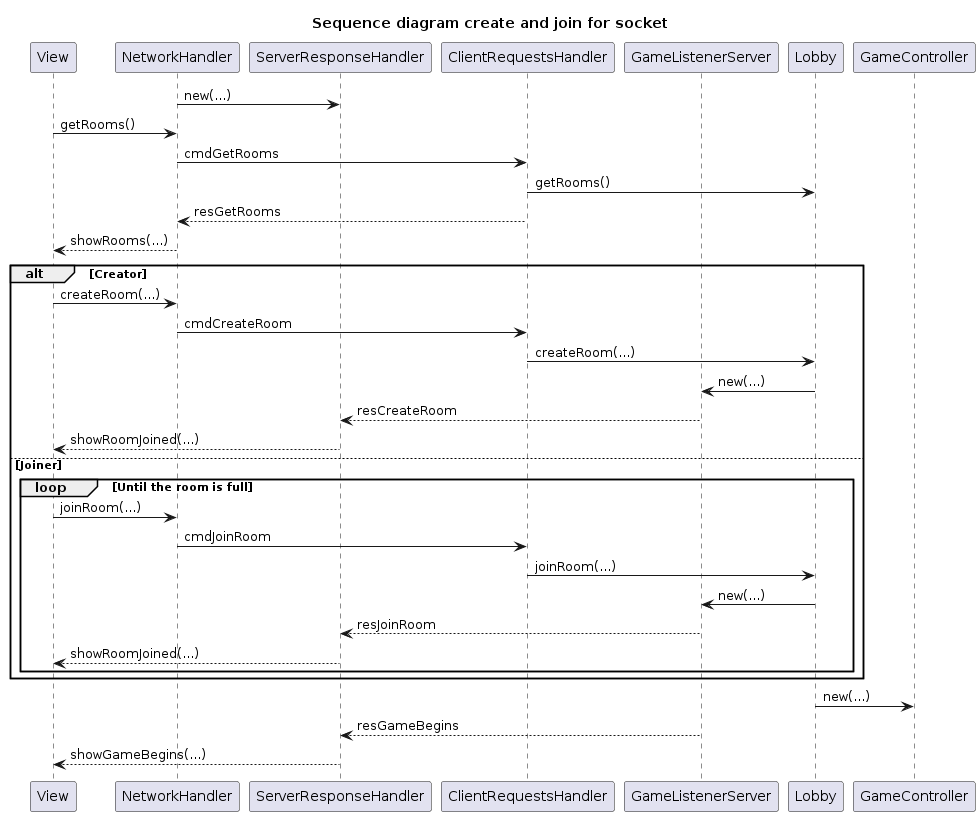
\includegraphics[width=0.9\textwidth]{img/sequenceRoomsDetailed.png}
  \caption{Sequence diagram per la popolazione della Room di gioco.}
  \label{fig:sequenceRooms}
\end{figure}

\subsubsection{Sequence diagram per la fase di inizializzazione del gioco}
Questa è la fase iniziale del gioco, in cui ogni giocatore deve fare le 2 scelte iniziali su come giocare la carta iniziale e quale carta obiettivo scegliere tra le 2 pescate.
\begin{figure}[H]
  \centering
  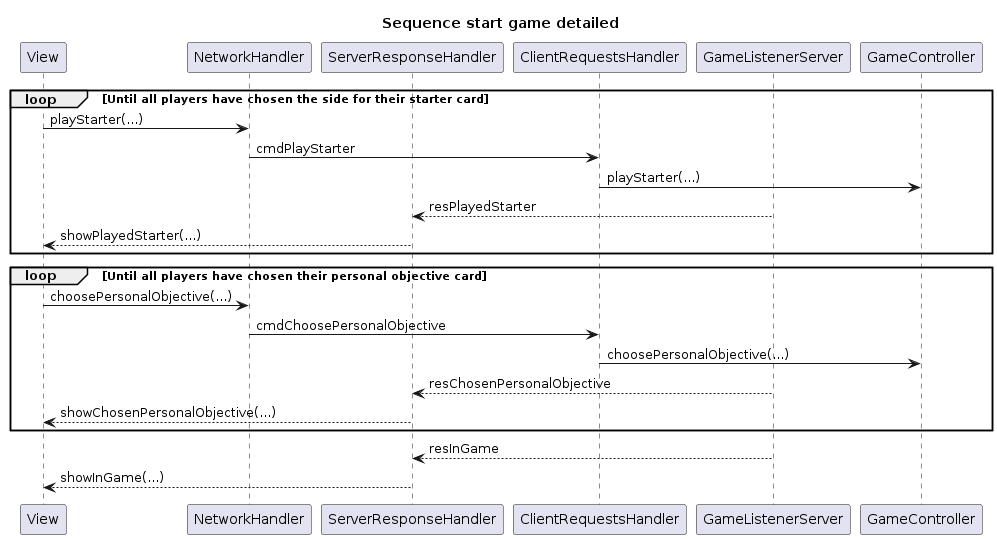
\includegraphics[width=0.9\textwidth]{img/sequenceStartGameDetailed.png}
  \caption{Sequence diagram dell'inizializzazione della partita.}
  \label{fig:sequenceStartGame}
\end{figure}

\subsubsection{Sequence diagram per la fase a turni del gioco, fino alla fine}
Questa è la fase a turni del gioco, nella quale i giocatori pescano e giocano le carte secondo l'ordine stabilito.
\\
Si distingue una prima sotto-fase che termina quando un giocatore ha raggiunto 20 punti oppure sono stati finiti entrambi i deck. In seguito vi è la fase finale in cui si completa il turno in corso e ciascun giocatore gioca un turno addizionale.
\\
Infine, vengono notificati a tutti i giocatori i loro punteggi aggioranti considerando le carte obiettivo, e il vincitore della partita.
\begin{figure}[H]
  \centering
  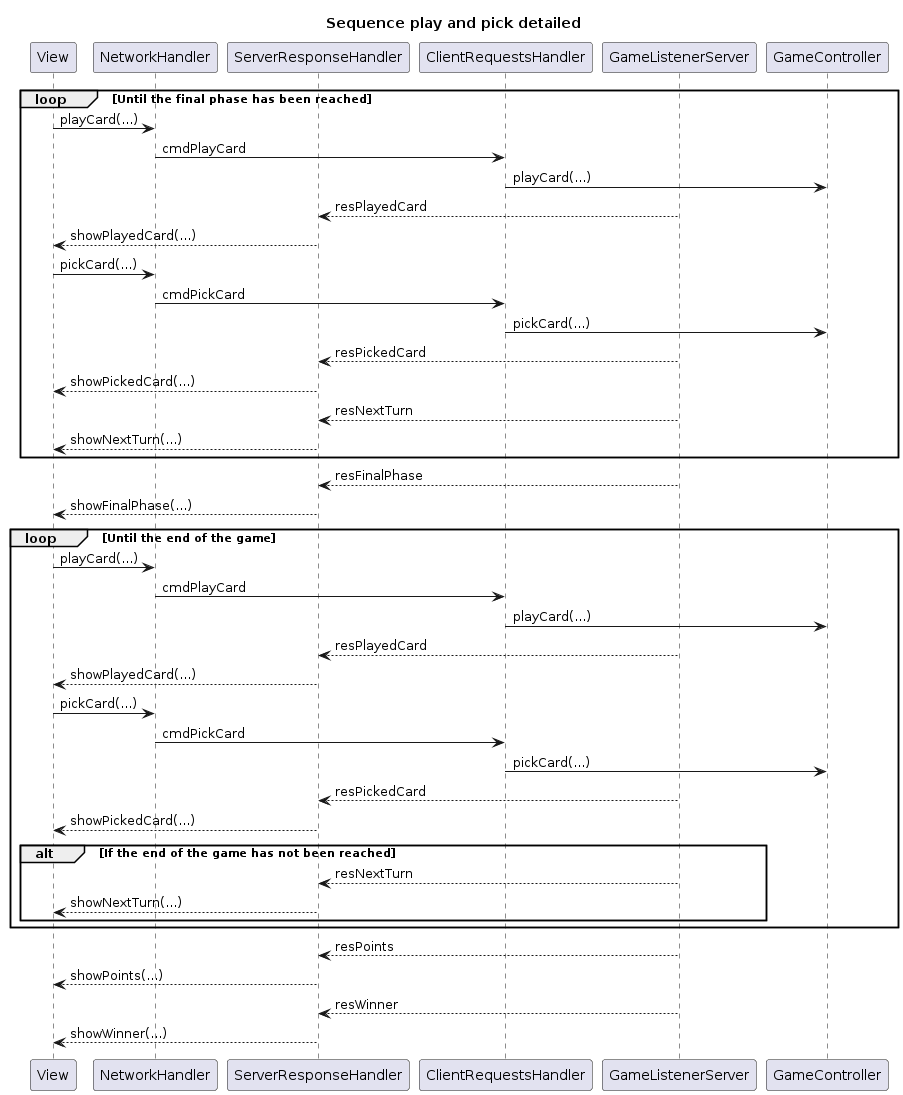
\includegraphics[width=0.9\textwidth]{img/sequenceTillTheEndDetailed.png}
  \caption{Sequence diagram della gestione del flusso di gioco.}
  \label{fig:sequenceTillTheEnd}
\end{figure}

\subsubsection{Sequence diagram per la sconnessione e riconnessione di un giocatore}
In queto sequence diagram mostriamo un esempio di sconnessione e riconnesione di un giocatore durante la fase a turni del gioco (per la relativa funzionalità avanzata).
\\
Anche se in questo esempio non è mostrato, abbiamo gestito la possibilità che resti solo un giocatore connesso. In tal caso si interrompe la partita e viene fatto partire un timer, allo scadere del quale si verifica il numero di giocatori connessi: se ce ne sono più di 1, la partita riprende; se ce n'è uno, viene decretato vincitore e viene terminata la partita; se non ce n'è nessuno, viene terminata la partita.
\begin{figure}[H]
  \centering
  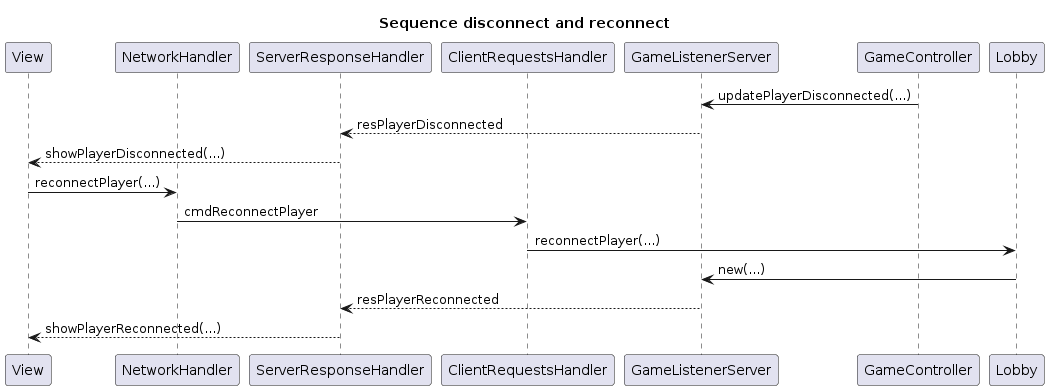
\includegraphics[width=0.9\textwidth]{img/sequenceDisconnectReconnectDetailed.png}
  \caption{Sequence diagram della per la sconnessione e riconnessione di un giocatore.}
  \label{fig:sequenceTillTheEnd}
\end{figure}

\section{RMI}
Abbiamo implementato anche la comunicazione tramite RMI, che nasconde la presenza della rete tra client e server. La struttura di base dei sequence diagram rimane inalterata, ma le classi intermedie che codificano e decodificano esplicitamente i pacchetti da mandare in rete sono sostituite da altre implementazioni di interfacce comuni che eseguono direttamente chiamate a metodi remoti. Si rimanda all'UML per tali implementazioni.

Così con RMI un generico evento client diventa una chiamata effettuata da \texttt{NetworkHandlerRMI} alle classi \texttt{LobbyRMI} o \texttt{GameControllerRMI} (gli oggetti remoti esposti dal server). Questo comporta una modifica dello stato del gioco, che verrà notificata tramite \texttt{ListenerHandler} alle corrispondenti classi \texttt{GameListenerServerRMI} (classi presenti nel server, uno per ogni client in gioco). Queste classi effettuano chiamate remote su \texttt{GameListenerClientRMI} (classi presenti nel client ed esposte come oggetti remoti in rete, corrispettive di quelle del server), che cambieranno lo stato del gioco per il client e quindi modificheranno la view.

L'unica eccezione a questo è il metodo \texttt{getRooms()} di \texttt{GameControllerRMI}, che ritorna direttamente la lista delle stanze

\end{document}
